\section{Optimizing the aTag Enhancements}


\subsection{Width with Variable Length Identifiers}
\subsubsection{Kraft's Inequality}
\subsubsection{Minimizing Kraft to Decrease Tag Width}


\subsection{Partial to Total Ordering}

Unfortunately, converting a partially ordered universe to a totally ordered universe is not straightforward. There can potentially be sets of incomparable elements, rather than just pairs, making it unclear which elements to split to resolve incomparabilities with the least number of additional bits. In the worst case where every pair of elements is incomparable, 

 Figure \ref{fig:ordering} shows one algorithm for doing so at a high level. For a concrete example, we are given four input sequences we wish to encode, shown in \ref{fig:ordering}(a). We assume that these sequences \textit{almost} follow an underlying ordering, but that there are a few incomparable sets of elements. In this example, $B$ is incomparable with $C$ because $B$ appears both before and after $C$. 

To systematically identify these incomparable elements, we construct the sequence graph, shown in \ref{fig:ordering}(b). In the sequence graph, element $u$'s node has an edge to element $v$'s node if $u$ appears before $v$ in any sequence. We then run an algorithm for finding Strongly Connected Components (SCCs) on this graph. A strongly connected component is a set of nodes such that for every pair of nodes $u$ and $v$ in the set, $u$ has a path to $v$ and vice versa. In this context, every SCC corresponds to a set of incomparable elements. Figure \ref{fig:conflict_res} shows the process for determining which elements to split to create a new, totally ordered universe. Figure \ref{fig:ordering}(d) and (e) shows the result of using this new ordering to modify each sequence. 


\begin{figure}[t!] 
\begin{minipage}{1\linewidth}
\begin{subfigure}[c]{0.96\linewidth}
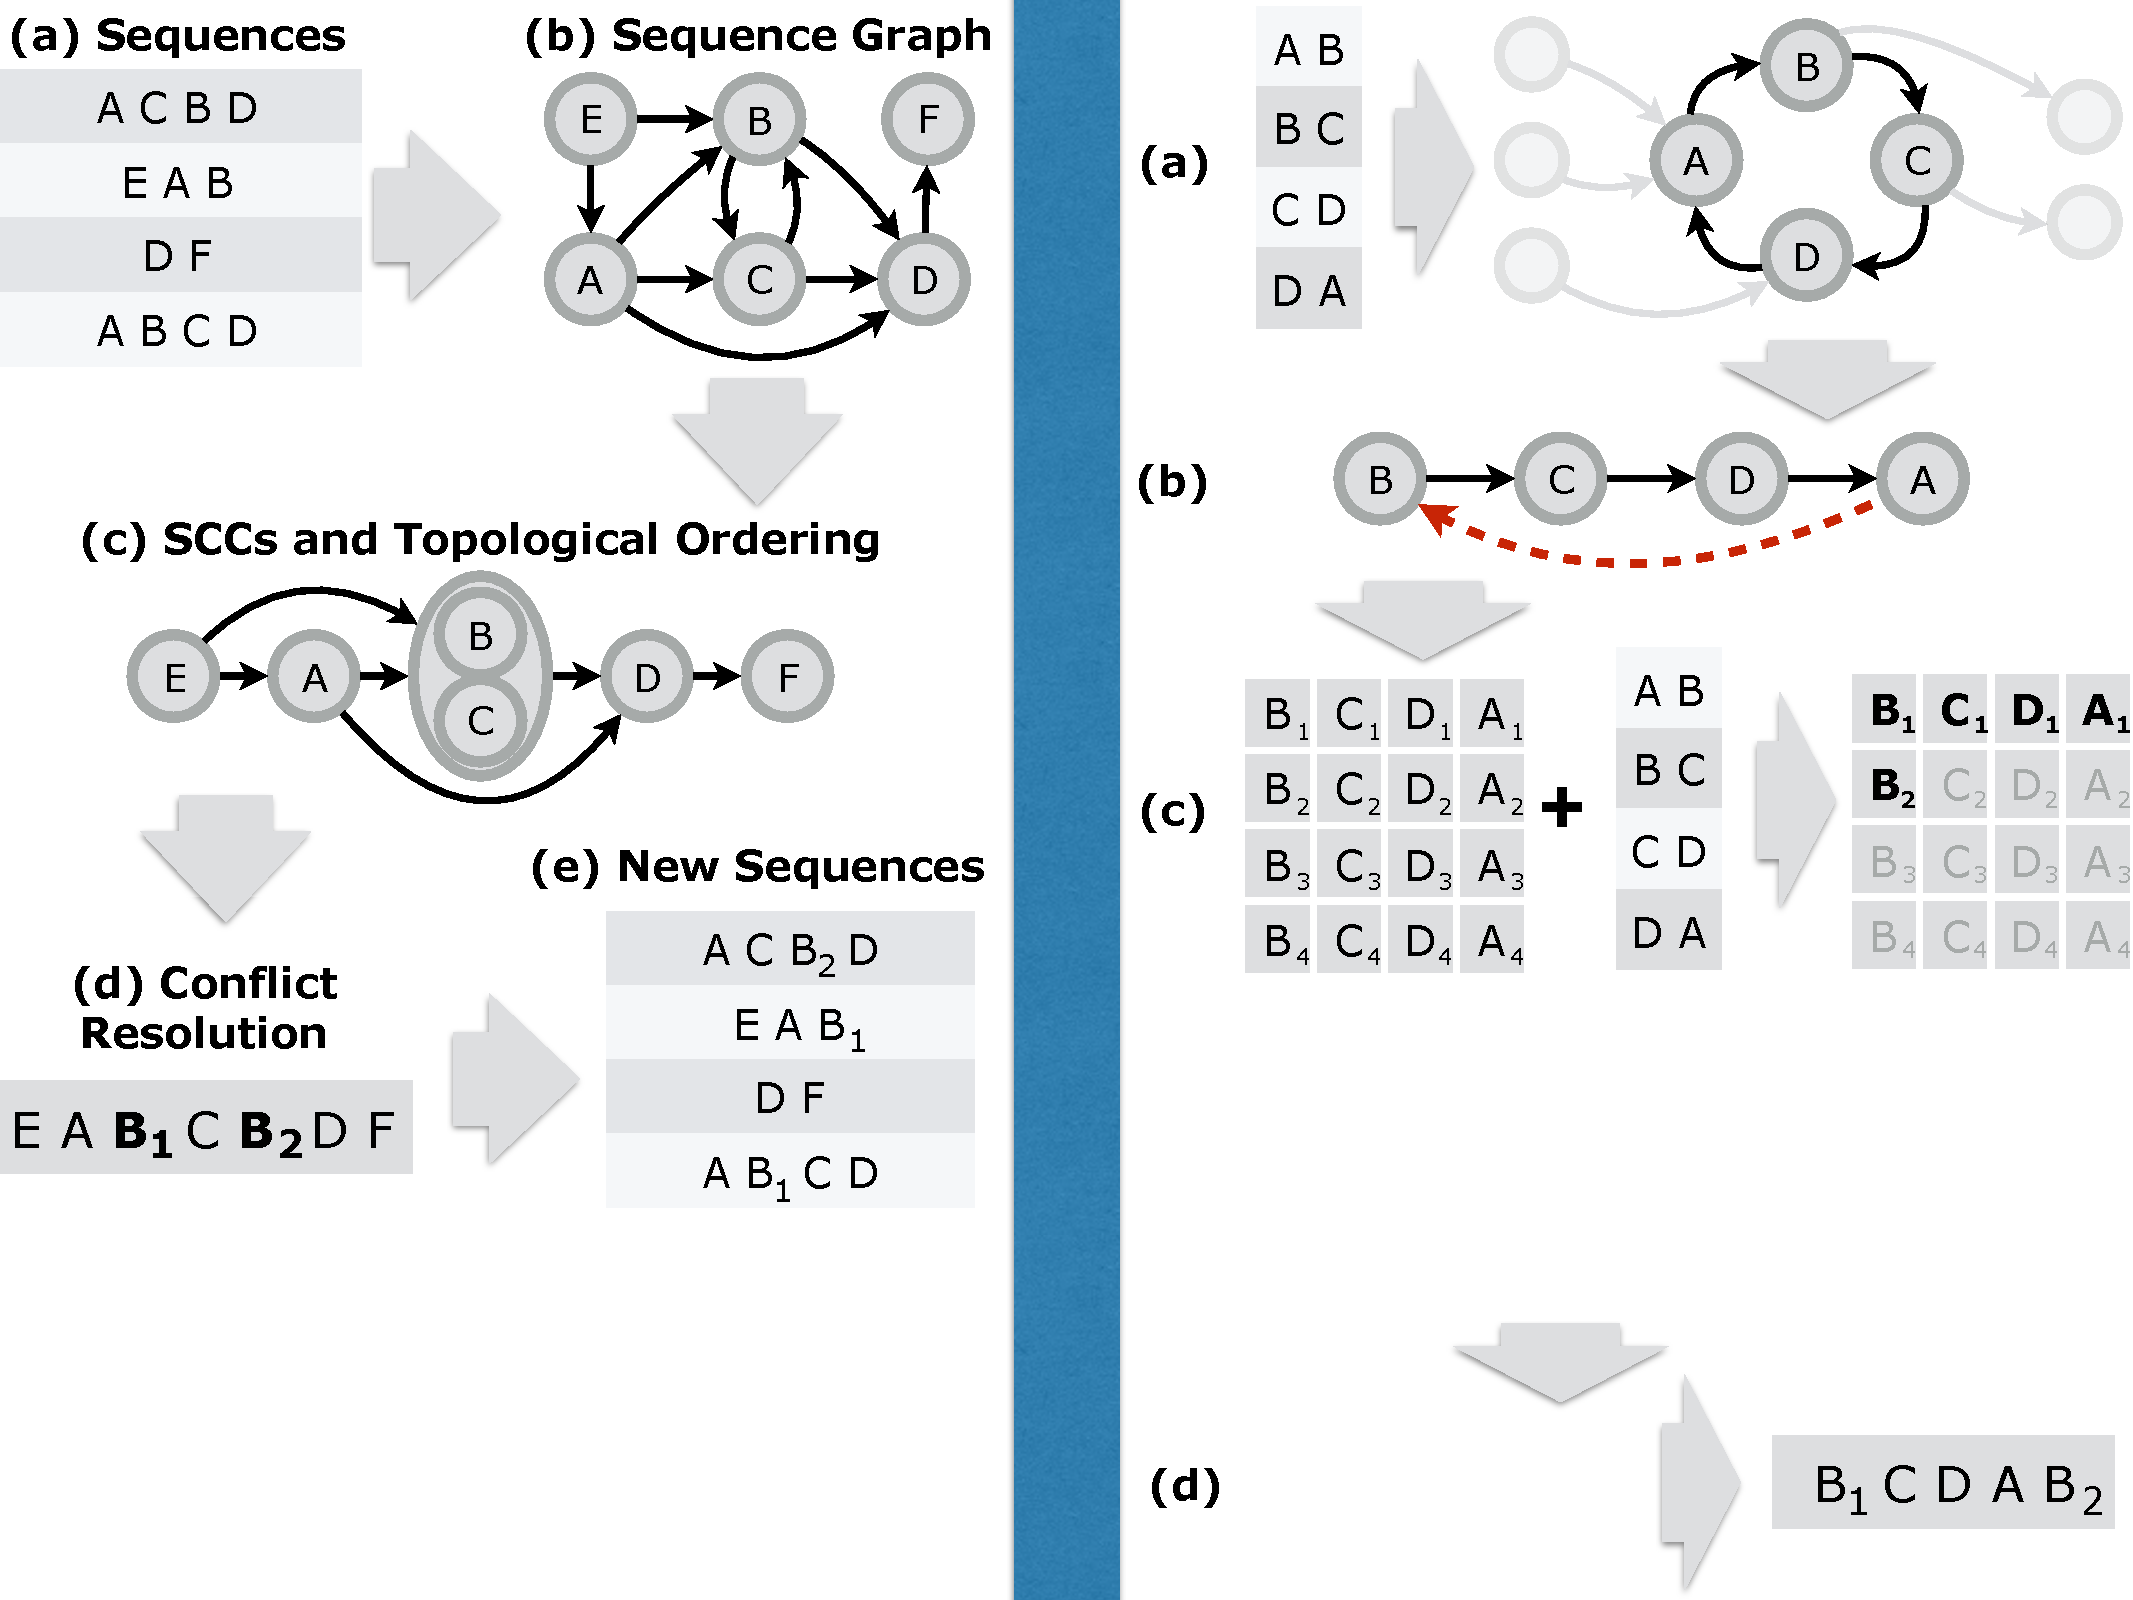
\includegraphics[trim={0 6cm 19.2cm 0}, clip, width=\linewidth]{figures/partial_ordering}
\end{subfigure} 
\end{minipage} 
\caption{This figure shows, at a high level, the process for converting a partial ordering to a total ordering by identifying incomparable elements and creating duplicates to resolve the incomparabilities. (a) shows the four input ordered sequences. In (b), we create a graph of the elements, where there is an edge from $u$ to $v$ if $u$ appears before $v$ in some sequence. (b) shows how the graph can be broken up into an ordered Directed Acyclic Graph (DAG) of Strongly Connected Components (SCC), where each SCC corresponds to a set of incomparable elements. (d) shows the result of splitting elements to resolve incomparability, which is covered in more depth in figure \ref{fig:conflict_res}. In (e), the original sequences are modified with the splits such that each sequence adheres to a total ordering.}
\label{fig:ordering}
\end{figure}



\begin{figure}[t!] 
\begin{minipage}{1\linewidth}
\begin{subfigure}[c]{0.96\linewidth}
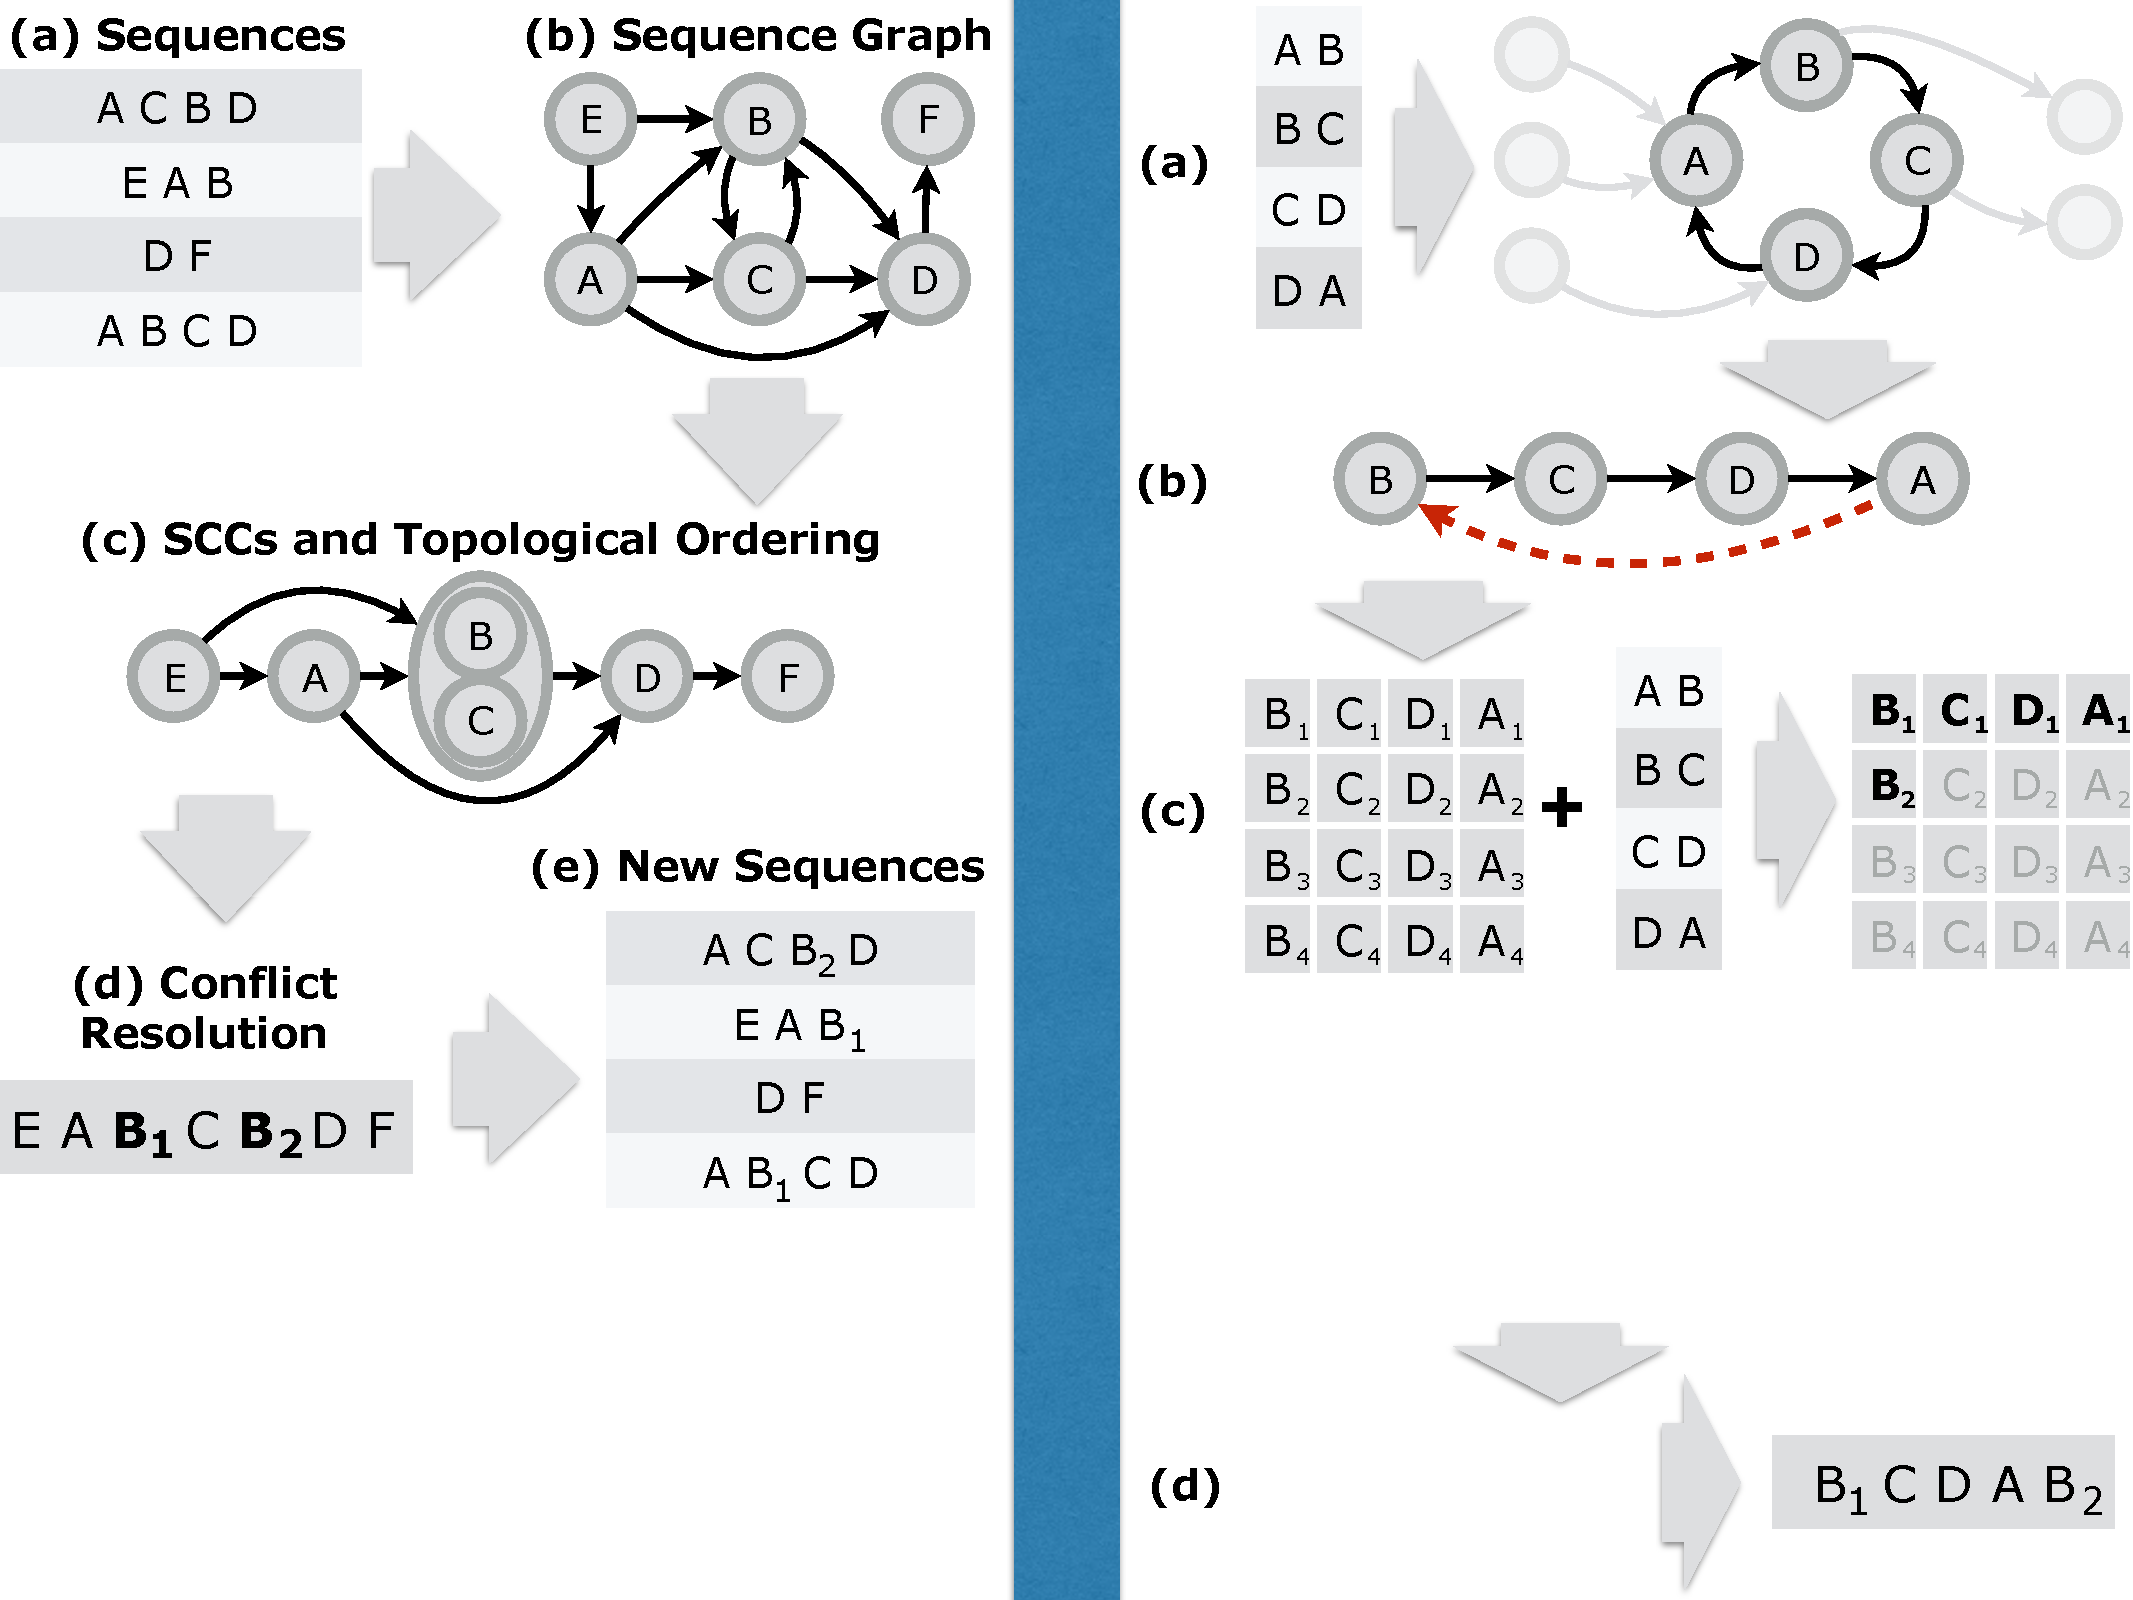
\includegraphics[trim={19.2cm 10cm 0 0}, clip, width=\linewidth]{figures/partial_ordering}
\end{subfigure} 
\end{minipage} 
\caption{This details the Conflict Resolution step of the algorithm. (a) shows a SCC corresponding to four incomparable elements. (b) shows an 'almost' ordering of the SCC nodes, which minimizes the number of backward edges. (c) shows how the almost ordering is used to construct a worst-case quadratically-sized universe, which is then traversed by every sequence to determine which splits are necessary. }
\label{fig:conflict_res}
\end{figure}